\documentclass[12pt]{article}
\usepackage[utf8]{inputenc}
\usepackage[T1]{fontenc}
\usepackage[spanish]{babel}
\usepackage{amsmath}
\usepackage{amssymb}
\usepackage{geometry}
\usepackage[backend=biber,style=numeric]{biblatex}
\usepackage{csquotes}
\addbibresource{referencias.bib}
\geometry{margin=1in}

\usepackage{listings}
\usepackage{xcolor}
\usepackage{graphicx} % Para insertar imágenes
\usepackage{subcaption} % Para poner varias imágenes juntas
\usepackage{float} % Para controlar la posición exacta [H]
\usepackage{hyperref}

\lstset{
    language=Python,
    basicstyle=\ttfamily\footnotesize,
    keywordstyle=\color{blue},
    commentstyle=\color{gray},
    stringstyle=\color{black},
    numbers=left,
    numberstyle=\tiny,
    frame=single,
    rulecolor=\color{black},
    breaklines=true,
    showstringspaces=false
}

\title{Actividad 3. Datos Sintéticos}
\author{Ing. Isaias Garcia Zanella}
\date{\today}

\begin{document}

\maketitle

\section{Introducción}
En el ámbito de la ciencia de datos, la disponibilidad de información es un requisito indispensable para el entrenamiento de modelos predictivos. Sin embargo, en sectores críticos como el de la salud, el acceso a datos reales suele estar restringido por normativas de privacidad y la sensibilidad de la información. Ante este escenario, el uso de datos sintéticos surge como una solución estratégica que permite generar representaciones matemáticas fieles sin vulnerar la confidencialidad de los pacientes.

El presente reporte detalla el desarrollo y validación de un conjunto de datos sintéticos hospitalarios. El objetivo principal fue escalar un conjunto de datos reducido a una base robusta de 1200 registros, empleando una metodología incremental en tres fases: individual, por parejas y grupal. A través de técnicas de selección probabilística y la aplicación de reglas de negocio basadas en sesgos institucionales, se busca demostrar que es posible expandir la densidad de los datos manteniendo la fidelidad estadística y la realidad clínica original.

\section{Marco Teórico}
\subsection{Datos Sinteticos}
    Los datos sinteticos, como su nombre lo indica, son datos que son creados artificialmente, en lugar
de ser obtenidos mediante mediciones o eventos. Generalmente, se utilizan algoritmos para aumentar el numero 
de datos, ya sea porque las pruebas requieren, o no existen suficientes instancias para entrenar un algoritmo.

Existen varias razones por las cuales los datos sinteticos son importantes, algunas de ellas son:
\begin{itemize}
    \item Cuando se requieren datos para prueba pero no estan disponibles en ese momento o no existen.
    \item Cuando se tiene una cantidad pequena de instancias y no alcanzan para hacer tanto el entrenamiento como las pruebas.
    \item Cuando se requieren datos de entrenamiento; sin embargo, es costoso o inviable realizarlos.
\end{itemize}

Existen muchos beneficios de crear y usar datos sinteticos. En muchas ocasiones, los desarrolladores necesitan la flexibilidad para poder probar un algoritmo y no se tienen todos los datos disponibles o se requiere
de mucho tiempo para poder adquirir y preparar suficientes datos.

Tambien se pueden hacer las pruebas cuando las clases estan desbalanceadas. Esto significa que hay muchas mas instancias que pertenecen a una clase , que a las demas. Esto para algunos algoritmos puede ser un problema y afecta su rendimiento, mientras que teniendo datos sinteticos se puede observar el rendimiento  de los algoritmos
mucho antes de hacer pruebas con los reales.

Otro beneficio de los datos sinteticos es la proteccion de datos reales mientras se trabaja con el modelo utilizando datos sinteticos. Para muchas aplicaciones los datos reales contienen informacion privada y sensible como datos biometricos, teledonos, direcciones, coordenadas de GPS en tiempo real, entre otros.

Existen diferentes tipos de datos sinteticos, los cuales tienen diversos propositos. En general se puede dividir de la siguiente manera:
\begin{itemize}
    \item Texto sintetico
    \item Datos sinteticos multimedia ( como videos , imagenes, sonidos,etcetera).
    \item Datos tabulares sinteticos.
\end{itemize}

Los textos sinteticos han sido un tema complejo hasta hace unos anos. Crear texto en un idioma que haga sentido, con las complejas reglas gramaticales que existen en practicamente cualquier idioma, no es una tarea simple, aunque hoy en dia, existen nuevos modelos de aprendizaje maquina que pueden generar texto conveniente bueno utilizando algoritmos de generacion de lenguaje natural.

Los datos sinteticos tambien pueden ser multimedia, como imagenes, video o sonidos. Usualmente, los datos sinteticos multimedia se cran utilizando entrenamiento - las redes profuncas,
por ejemplo, suelen utilizar un gran numero de datos y,si se esta utilizando un algoritmo para, por ejemplo, clasificar imagenes, en ocasiones, se requieren de una mayor cantidad de datos- o para reemplazar datos multimedia sensibles o confidenciales- por ejemplo, los datos biometricos, como se comento anteriormente-.
~\cite{De0a100enIA}

% \subsection{Método de la Ruleta}
% El método de la ruleta es una técnica utilizada en algoritmos genéticos para seleccionar individuos de una población en función de su aptitud (*fitness*) para formar parte de la siguiente generación. Los pasos para implementar este método en la generación de datos sintéticos son los siguientes:

% \begin{itemize}
%     \item \textbf{Generación de datos iniciales:} Crear una muestra de datos sintéticos que represente el problema que se está tratando de resolver. Es posible generar datos aleatorios o seguir una distribución específica según las características que se deseen simular.
%     \item \textbf{Definición de la función de aptitud:} Para aplicar el método de la ruleta, se debe contar con una función que evalúe la calidad o "aptitud" de cada individuo (punto de datos) dentro de la población.
%     \item \textbf{Cálculo de la aptitud:} Aplicar la función de aptitud a cada punto de la población sintética para obtener sus respectivos valores numéricos.
%     \item \textbf{Normalización de la aptitud:} Es fundamental que los valores de aptitud sean no negativos y, preferiblemente, mayores que cero. Se pueden utilizar técnicas como la escala min-max para asegurar que todos los valores sean comparables.
%     \item \textbf{Cálculo de probabilidades de selección:} Convertir los valores de aptitud normalizados en probabilidades. La probabilidad de cada individuo es proporcional a su aptitud respecto al total de la población.
%     \item \textbf{Construcción de la ruleta:} Crear una "ruleta" ficticia acumulando las probabilidades en una lista o arreglo. Cada intervalo de probabilidad acumulada representa un sector de la ruleta; entre mayor sea la aptitud, mayor será el sector asignado.
%     \item \textbf{Selección de individuos:} Generar números aleatorios entre 0 y 1 para seleccionar a los individuos. El número aleatorio actúa como el "tiro" de la ruleta, y el individuo cuyo intervalo de probabilidad acumulada contenga dicho número será el elegido.
%     \item \textbf{Repetición del proceso:} Repetir la selección y reproducción durante varias generaciones para evolucionar la población sintética hacia soluciones más óptimas o adecuadas para el problema específico de ciencia de datos. 
% \end{itemize}
% ~\cite{De0a100enIA}
\subsection{Metodo de Ruleta}
El metodo de la ruleta es una tecnica utilizada en algoritmos geneticos para seleccionar individuos de una poblacion en funcion de su aptitud para ser parte de la siguiente generacion. Los pasos para implementar el metodo de la ruleta para generar datos sinteticos, son los siguientes:
\begin{itemize}
    \item \textbf{Generacion de datos sinteticos:} Crea una muestra de datos sinteticos que presente el problema que esta tratando de resolver. Puedes generar datos aleatorios o seguir una distribución específica según las características que deseas simular.
    \item \textbf{Definicion de funcion de aptitud:} Para aplicar el metodo de la ruleta, debes de tener una funcion que evalue la aptitud de cada individuo (punto de datos) en la poblacion.
    \item \textbf{Calculo de la aptitud de cada individuo:} Aplica la funcion de aptitud a cada punto de datos de la población sintética para obtener sus respectivos valores de aptitud.
    \item \textbf{Normalizacion de la aptitud:} Asegurate de que los valores de aptitud sean todos no negativos y, preferiblemente, mayores que cero. Puedes usar tecnicas de normalización, como la escala min-max o la normalización Z-score, para lograrlo.
    \item \textbf{Calculo de probabilidades de seleccion:} Convierte los valores de aptitud normalizados en probabilidades de selección para cada individuo.
    \item \textbf{Creacion de ruleta: } Construye una ruleta ficticia utilizando las probabilidades de seleccion calculadas. Esto se puede hacer acumulando las probabilidades en una lista o un arreglo, donde cada intervalo de probabilidad respresenta un sector en la ruleta.
    \item \textbf{Seleccion de individuos: } Lanza una serie de numeros aleatorios para seleccionar los individuos de la polacion sintetica. Cada numero aleatorio representa una tirada de la ruleta, y el individuo cuya probabilidad acumulada corresponda al numero seleccionado sera elegido.
    \item \textbf{Repreticion del proceso: } Repite el proceso de seleccion y reproduccion durante varias generaciones para evolucionar la poblacion sintetica hacia soluciones mas optimas o apropiadas para tu problema especifico de ciencia de datos. 
\end{itemize}
~\cite{De0a100enIA}

% Información complementaria agregada
\textbf{Consideraciones adicionales sobre la selección proporcional:}
Para que la selección sea matemáticamente consistente, la probabilidad de elección $P_i$ de cada individuo debe cumplir con la relación $P_i = f_i / \sum_{j=1}^{N} f_j$. Un aspecto crítico a considerar es el riesgo de la \textit{convergencia prematura}, la cual ocurre cuando un individuo con aptitud sobresaliente domina rápidamente la ruleta, reduciendo la diversidad genética. Para mitigar esto, se recomienda el uso de mecanismos de escalamiento de aptitud o el algoritmo de \textit{Muestreo Universal Estocástico} (SUS), el cual reduce la varianza en la selección al utilizar un único disparo de ruleta con múltiples punteros equidistantes~\cite{Eiben2015}.

% \subsection{Metodo SMOTE}
% El metodo SMOTE( Syntethic Minority Over-sampling Technique) es una tecnica utilizada en el campo del aprendizaje automatico para crear datos sinteticos y equilibrar conjuntos de datos desequilibrados. Se utiliza especialmente cuando se tiene una clase minoritaria co pocas instancias y una clase mayoritaria con muchas instancias.


% SMOTE funciona tomando ejemplos de la clase minoritaria y generando ejemplos sinteticos interpolando caracteristicas entre estos ejemplos existentes. Basicamente, se seleccionan dos ejemplos cercanos en el espacio de caracteristicas y se crea un nuevo ejemplo tomando una combinacion ponderada de sus atributos. Este proceso se repite varias veces hasta que se genera la cantidad deseada de ejemplos sinteticos.

% Los pasos para implementar SMOTE como tecnica de datos sinteticos son los siguientes:
% \begin{itemize}
%     \item Preparacion de los datos. Primero, se tiene que lidiar con los valores faltantes y todo lo necesario con respecto a preprocesamiento.
%     \item Entender el desequilibrio de clases. Es importante realizar un analisis para comprender el grado de desequilibrio en el conjunto de datos. Es importante saber que tan grande es la brecha entre las clases mayoritaria y minoritaria.
%     \item Division del conjunto de datos. Se debe separar el conjunto de datos en dos conjuntos: uno para entrear el modelo y otro para evaluar el rendimiento posteriormente. El conjunto de entrenamiento sera utilizado para aplicar SMOTE.
%     \item Aplicar SMOTE al conjunto de entrnamiento. Se deben generar instancias sinteticas de acuerdo al muestreo que realizo la interpolacion por SMOTE.
% \end{itemize}

% Consideraciones adicionales: 
% \begin{itemize}
%     \item SMOTE puede generar instancias sinteticas, pero no garantiza que estas instancias sean realistas o validas para todos los conjuntos de datos. 
%     \item Si el desequilibrio de clases es extremadamente alto, SMOTE puede no ser suficiente para resolver el problema, y es posible que se deba considerar otras tecnicas mas avanzadas o estrategias de modificacion del algoritmo.
%     \item El exito de SMOTE y otras tecnicas de equilbrio de clases depende en gran medida del conjunto de datos y del problema especifico que estes abonando.
% \end{itemize}

% Ventajas de SMOTE:
% \begin{itemize}
%     \item Soluciona el problema de desequilibrio de clases al generar ejemplos sinteticos de la clase minoritaria, lo que ayuda a mejorar el rendimiento del modelo en la prediccion de dicha clase.
%     \item Evita la perdida de informacion al generar datos sinteticos en lugar de duplicar ejemplos existentes, lo que puede conducir a un sobreajuste.
% \end{itemize}

% Desventajas de SMOTE:
% \begin{itemize}
%     \item Puede generar ejemplos sinteticos que no sean realistas o no se ajusten bien a la distribucion original de los datos, lo que podria afectar negativamente la precision del modelo.
%     \item Si los ejemplos de la clase minoritaria estan demasiado cerca o superpuestos en el espacio de caracteristicas, SMOTE puede generar ejemplos sinteticos que son muy similares entre si, lo que podria introducir sesgos en el conjunto de datos.
% \end{itemize}
% ~\cite{De0a100enIA}
\subsection{Metodo SMOTE}
El metodo SMOTE (Synthetic Minority Over-sampling Technique) es una tecnica utilizada en el campo del aprendizaje automatico para crear datos sinteticos y equilibrar conjuntos de datos desequilibrados. Se utiliza especialmente cuando se tiene una clase minoritaria con pocas instancias y una clase mayoritaria con muchas instancias.

SMOTE funciona tomando ejemplos de la clase minoritaria y generando ejemplos sinteticos interpolando caracteristicas entre estos ejemplos existentes. Basicamente, se seleccionan dos ejemplos cercanos en el espacio de caracteristicas y se crea un nuevo ejemplo tomando una combinacion ponderada de sus atributos. Este proceso se repite varias veces hasta que se genera la cantidad deseada de ejemplos sinteticos.

A diferencia del sobremuestreo aleatorio (\textit{Random Over-sampling}), que simplemente duplica instancias existentes, SMOTE crea nuevos puntos de datos en el segmento de línea que une a los $k$ vecinos más cercanos de la clase minoritaria. Matemáticamente, si $x_i$ es una instancia de la clase minoritaria y $x_{zi}$ es uno de sus vecinos más cercanos, la nueva instancia $x_{new}$ se calcula como:
\begin{equation}
    x_{new} = x_i + \lambda \times (x_{zi} - x_i)
\end{equation}
donde $\lambda$ es un número aleatorio entre 0 y 1. Este enfoque permite que el modelo aprenda fronteras de decisión más amplias y generales~\cite{Chawla2002}.

Los pasos para implementar SMOTE como tecnica de datos sinteticos son los siguientes:
\begin{itemize}
    \item \textbf{Preparacion de los datos:} Primero, se tiene que lidiar con los valores faltantes y todo lo necesario con respecto a preprocesamiento.
    \item \textbf{Entender el desequilibrio de clases:} Es importante realizar un analisis para comprender el grado de desequilibrio en el conjunto de datos. Es importante saber que tan grande es la brecha entre las clases mayoritaria y minoritaria.
    \item \textbf{Division del conjunto de datos:} Se debe separar el conjunto de datos en dos conjuntos: uno para entrenar el modelo y otro para evaluar el rendimiento posteriormente. El conjunto de entrenamiento sera utilizado para aplicar SMOTE.
    \item \textbf{Aplicar SMOTE al conjunto de entrenamiento:} Se deben generar instancias sinteticas de acuerdo al muestreo que realizo la interpolacion por SMOTE.
\end{itemize}

Consideraciones adicionales: 
\begin{itemize}
    \item SMOTE puede generar instancias sinteticas, pero no garantiza que estas instancias sean realistas o validas para todos los conjuntos de datos. 
    \item Si el desequilibrio de clases es extremadamente alto, SMOTE puede no ser suficiente para resolver el problema, y es posible que se deba considerar otras tecnicas mas avanzadas o estrategias de modificacion del algoritmo, como SMOTE-Tomek o SMOTE-ENN, que combinan el sobremuestreo con la limpieza de datos ruidosos~\cite{Batista2004}.
    \item El exito de SMOTE y otras tecnicas de equilbrio de clases depende en gran medida del conjunto de datos y del problema especifico que estes abordando.
\end{itemize}

Ventajas de SMOTE:
\begin{itemize}
    \item Soluciona el problema de desequilibrio de clases al generar ejemplos sinteticos de la clase minoritaria, lo que ayuda a mejorar el rendimiento del modelo en la prediccion de dicha clase.
    \item Evita la perdida de informacion al generar datos sinteticos en lugar de duplicar ejemplos existentes, lo que puede conducir a un sobreajuste (\textit{overfitting}).
\end{itemize}

Desventajas de SMOTE:
\begin{itemize}
    \item Puede generar ejemplos sinteticos que no sean realistas o no se ajusten bien a la distribucion original de los datos, lo que podria afectar negativamente la precision del modelo.
    \item Si los ejemplos de la clase minoritaria estan demasiado cerca o superpuestos en el espacio de caracteristicas, SMOTE puede generar ejemplos sinteticos que son muy similares entre si o que invaden el espacio de la clase mayoritaria, lo que podria introducir sesgos o ruido en el conjunto de datos.
\end{itemize}
~\cite{De0a100enIA}

\subsection{Metodo ADASYN}
El metodo ADASYN (Adaptative Syntethic Sampling) es una tecnica utilizada en el aprendizaje automatico para tratar el desequilibrio de clases en conjuntos de datos.

Es una forma generalizada del algoritmo SMOTE. La idea es generar adaptativamente muestras de datos en funcion de sus distribuciones, es decir, generar datos sinteticos para la muestras de las clase minoritaria que son mas dificiles de aprender, en comparacion con las muestras minoritarias que son faciles de aprender.

Las etapas basicas para implementar el metodo ADASYN de manera sencilla son las siguientes:
\begin{enumerate}
    \item \textbf{Preparacion de los datos:} Comienza por asegurarse de tener un conjunto de datos desequilibrados, es decir, con una clase minoritaria y una clase mayoritaria. Asegurate de tener las caracteristicas de tus datos y las etiquetas que indican las clases a las que pertenecen.
    \item \textbf{Determinar el grado de desequilibrio:} Calcula la diferencia entre el numero de muestras de la clase mayoritaria y la clase minoritaria. Esto te ayudara a comprender que tan desequilibrado esta tu conjunto de datos y que tan sinteticos deben ser los datos generados.
    \item \textbf{Calcular la tasa de generacion sintetica: } La tasa de generacion sintetica es un parametro que determina cuantos datos sinteticos se deben generar en relacion con el numero de datos de la clase minoritaria.
    \item \textbf{Seleccionar una muestra de la clase minoritaria: } Comienza seleccionado aleatoriamnente una muestra de la clase minoritaria en tu conjunto de datos existente.
    \item \textbf{Calcular las distancias:} Calcula la distancia entre la muestra seleccionada y todas las demas muestras de la clase minoritaria.
    \item \textbf{Calcular la densidad relativa: } Calcula la densidad realtiva de cada muestra de la clase minoritaria dividiendo el numero de muestras de la clase mayoritaria dentro de cierta vecindad por el numero total de muestras en cada vecindad.
    \item \textbf{Calcular los pesos: } Calcula los pesos para cada muestra de la clase minoritaria basados en su densidad relativa. Los pesos se utilizan para determinar cuantos datos sinteticos se generan a partir de cada muestra.
    \item \textbf{Generar datos sinteticos: }Utilizando los pesos calculados en el paso anterior, genera nuevos datos sinteticos en las regiones de baja densidad de la clase minoritaria.
    \item \textbf{Combinar datos:} Combina los datos originales con los  datos sinteticos generados para obtener un nuevo conjunto de datos equilibrado.
\end{enumerate}
~\cite{De0a100enIA}

\section{Materiales y Métodos}

El desarrollo experimental se dividió en cuatro fases secuenciales: pre-procesamiento de datos, generación de datos sintéticos controlada, integración multiequipo y validación estadística. El entorno de desarrollo utilizado fue un Jupyter Notebook basado en el lenguaje Python 3.x, empleando las bibliotecas \texttt{pandas} para manipulación de estructuras, \texttt{numpy} para computación numérica y \texttt{seaborn} para el análisis visual.

\subsection{Fase 1: Definición de Sesgos y Carga de Datos}
Inicialmente, se cargó el dataset original mediante una función robusta de lectura. Posteriormente, se estableció un marco normativo denominado \texttt{config\_sesgos}, el cual define los límites técnicos para las variables críticas de cada institución.

\begin{lstlisting}[language=Python, caption={Carga de datos y reglas de negocio}]
def load_data_local(ubicacion):
    try:
        return pd.read_csv(ubicacion)
    except Exception as e:
        print(f"Error al cargar la B.D.: {e}")
        return None

# Definicion de rangos permitidos por hospital
config_sesgos = {
    'Hospital A': {
        'mortality_rate_30day': {'min': 0.10, 'max': 0.15},
        'readmission_rate_30day': {'min': 0.08, 'max': 0.12}
    }
}
\end{lstlisting}

\subsection{Fase 2: Generación por Algoritmo de Ruleta Validada}
Para aumentar el volumen de la muestra, se implementó un algoritmo de selección por ruleta. Este método selecciona registros base con probabilidad uniforme y los somete a una validación contra el diccionario de sesgos. Solo los registros que cumplen con las restricciones de mortalidad y readmisión son incorporados al nuevo conjunto de datos.

\begin{lstlisting}[language=Python, caption={Algoritmo de aumento y validacion de integridad}]
def aumentar_ruleta_con_validacion(df, n_deseado, reglas_hospitales):
    datos_validados = []
    probabilidades = np.ones(len(df)) / len(df)
    mapa_ids = df.set_index('hospital_name')['hospital_id'].to_dict()

    while len(datos_validados) < n_deseado:
        candidato = df.sample(n=1).iloc[0].copy()
        nombre = str(candidato['hospital_name']).strip()
        
        if nombre in reglas_hospitales:
            reglas = reglas_hospitales[nombre]
            if all(reglas[c]['min'] <= candidato[c] <= reglas[c]['max'] for c in reglas):
                candidato['hospital_id'] = mapa_ids.get(nombre, candidato['hospital_id'])
                datos_validados.append(candidato)
    
    df_nuevos = pd.DataFrame(datos_validados).reset_index(drop=True)
    return pd.concat([df, df_nuevos], ignore_index=True), df_nuevos
\end{lstlisting}

\subsection{Fase 3: Integración de Datos Multiequipo}
Con el objetivo de consolidar una base de datos global, se integraron los resultados del \textbf{Equipo 1} y el \textbf{Equipo 2}. El proceso de fusión consistió en una concatenación de DataFrames seguida de un reordenamiento jerárquico por identificador de hospital para garantizar la consistencia en el acceso a la información.

\begin{lstlisting}[language=Python, caption={Fusion de datos Equipo 1 y Equipo 2}]
# Union de resultados y limpieza
df_union = pd.concat([df_equipo1, df_equipo2], ignore_index=True)
df_union = df_union.sort_values(by=['hospital_id']).reset_index(drop=True)
\end{lstlisting}

\subsection{Fase 4: Evaluación de Distribuciones (KDE)}
La validación final se realizó mediante un análisis comparativo de la función de densidad de kernel (KDE). Se implementó un ciclo automatizado para contrastar el dataset original contra el dataset fusionado, asegurando que el incremento en la densidad de datos no alterara las tendencias centrales del problema inicial.

\begin{lstlisting}[language=Python, caption={Visualizacion de convergencia estadistica}]
def graficar_diferencia_datos(df_orig, df_union, col):
    plt.figure(figsize=(10, 6))
    sns.kdeplot(df_orig[col], label='Original', fill=True, alpha=0.3)
    sns.kdeplot(df_union[col], label='Union (Eq1+Eq2)', linestyle='--', color='red')
    plt.legend()
    plt.show()

# Validacion de todas las variables numericas
for columna in df_original.columns:
    if pd.api.types.is_numeric_dtype(df_original[columna]):
        graficar_diferencia_datos(df_original, df_union, columna)
\end{lstlisting}

\subsection{Metodología de Generación y Validación de Datos Sintéticos}

El proceso de expansión del conjunto de datos se llevó a cabo siguiendo una estrategia de validación incremental, asegurando que los sesgos hospitalarios definidos inicialmente se preservaran en cada etapa. A continuación se detallan las fases realizadas:

\begin{enumerate}
    \item \textbf{Generación Individual (Muestra Inicial de 150 registros):} 
    En la primera etapa, cada integrante del equipo generó un conjunto base de \textbf{150 datos sintéticos}. Para esto se utilizó el \textbf{método de selección por ruleta}, el cual permite realizar un muestreo probabilístico del dataset original. Cada dato generado fue sometido a una validación estricta frente a un diccionario de sesgos predefinido, garantizando que variables como la tasa de mortalidad y readmisión se mantuvieran dentro de los rangos médicos lógicos de cada institución.

    \item \textbf{Integración por Parejas (Consolidación de 300 registros):} 
    Posteriormente, el grupo se dividió en parejas para fusionar sus muestras individuales, logrando un dataset combinado de \textbf{300 registros}. El objetivo de esta fase fue evaluar la estabilidad del algoritmo al unir diferentes fuentes de datos sintéticos. Se realizaron pruebas de densidad (KDE) para comparar estos 300 datos contra el dataset original, verificando que la unión no desplazara las medias ni alterara significativamente la varianza de las métricas de salud.

    \item \textbf{Validación Grupal y Análisis de Desviación:} 
    Como paso final, se contrastó el dataset de 300 registros de cada equipo con los resultados obtenidos , dando un total de 1200 datos, por el resto de los grupos. Esta comparativa global permitió observar la \textbf{desviación existente} entre los datos originales y el total de los nuevos datos sintéticos generados. Este análisis es fundamental para identificar si el proceso de aumento de datos introdujo algún sesgo sistémico o si, por el contrario, los datos sintéticos son representaciones fieles y robustas de la población original.
\end{enumerate}

\section{Resultados y Discusión}

\section*{Fase 1: Generación de Datos Sintéticos}

El proceso de expansión del conjunto de datos se diseñó para garantizar que los modelos de aprendizaje automático posteriores cuenten con una base robusta y estadísticamente fiel a la realidad hospitalaria. A continuación, se detalla el desarrollo y los hallazgos de esta primera etapa.

\subsection*{1. Metodología de Generación Individual (150 datos)}
En esta etapa inicial, cada integrante del equipo generó un conjunto base de \textbf{150 registros sintéticos}. Se implementó un \textbf{método de selección por ruleta}, el cual permite realizar un muestreo probabilístico del dataset original. Para asegurar la coherencia médica y el realismo de los datos, cada registro generado fue validado frente a un diccionario de sesgos institucionales, filtrando aquellos que no cumplieran con los rangos lógicos de mortalidad y readmisión definidos para cada hospital.

\subsection*{2. Análisis de Resultados: Validación de la Muestra Inicial}
Tras la generación de los registros, se procedió a realizar una comparación visual mediante \textit{Kernel Density Estimation} (KDE) para contrastar los datos sintéticos frente a los originales. Las observaciones clave son:

\begin{itemize}
    \item \textbf{Fidelidad Estadística:} Como se observa en las gráficas de densidad (ver Figura \ref{fig:kde_fase1}), la distribución de los datos sintéticos (línea roja punteada) replica con alta precisión la tendencia de los datos originales (línea azul). Esto valida que el algoritmo de ruleta no altera la naturaleza probabilística de las variables críticas.

    \begin{figure}[H]
         \centering
         \begin{subfigure}[b]{0.48\textwidth}
             \centering
             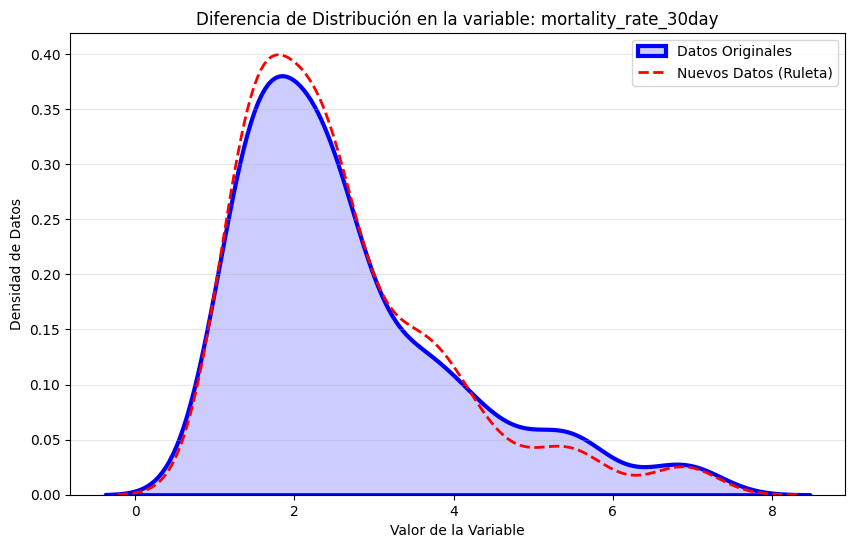
\includegraphics[width=\textwidth]{../Imagenes/Tarea3/Fase1_Mortalidad_30dias.png}
             \caption{Tasa de Mortalidad a 30 días}
         \end{subfigure}
         \hfill
         \begin{subfigure}[b]{0.48\textwidth}
             \centering
             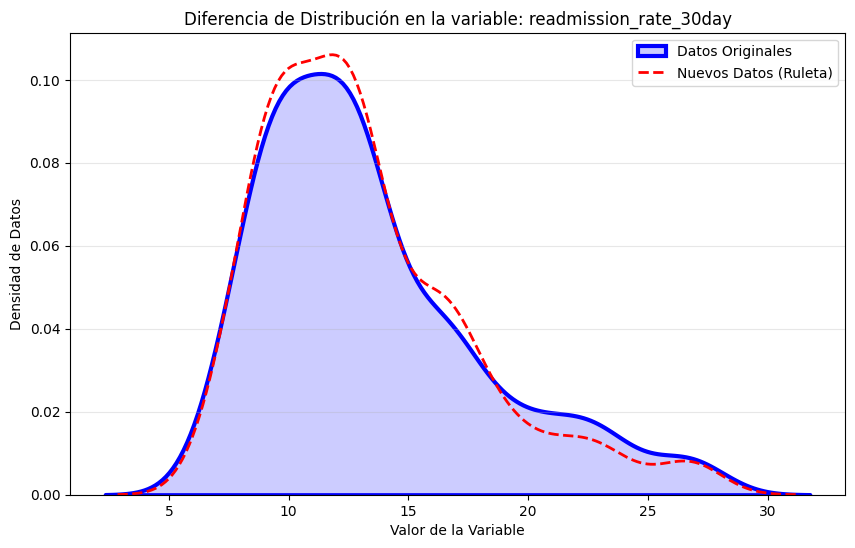
\includegraphics[width=\textwidth]{../Imagenes/Tarea3/Fase1_TasaReadmision.png}
             \caption{Tasa de Readmisión a 30 días}
         \end{subfigure}
         \caption{Comparativa de densidades KDE: Datos Originales (azul) frente a Datos Sintéticos (rojo) para la muestra individual de 150 registros.}
         \label{fig:kde_fase1}
    \end{figure}
    

    \item \textbf{Preservación de Sesgos:} Los picos de frecuencia (modas) se mantienen en los mismos rangos porcentuales en ambas curvas. Esto confirma que el conocimiento experto volcado en el diccionario de sesgos se transfirió correctamente al nuevo dataset, respetando las particularidades de cada hospital.
    
    \item \textbf{Estabilidad para la Integración:} La varianza observada en la muestra de 150 datos es controlada y no presenta valores atípicos significativos, lo que proporciona una base sólida para la siguiente fase de integración.
\end{itemize}

\section*{Fase 2: Integración y Consolidación de Resultados (300 registros)}

Tras la validación individual, se procedió a la unión de los datasets generados por los integrantes del equipo, alcanzando un total de \textbf{300 registros sintéticos}. Esta fase permitió evaluar la estabilidad del algoritmo al manejar un mayor volumen de información.

\subsection*{1. Análisis de Resultados: Estabilidad de la Unión}
Al contrastar el dataset consolidado de 300 registros contra el dataset original (ver Figura \ref{fig:kde_fase2_completa}), se identificaron los siguientes puntos clave:

\begin{itemize}
    \item \textbf{Convergencia de Distribuciones:} La curva sintética (roja) muestra una superposición casi total con la original (azul). El incremento de la muestra permitió que el algoritmo de ruleta capturara con mayor precisión las modas de cada variable.
    \item \textbf{Suavizado Estadístico:} Se observa una reducción significativa del ruido en comparación con la Fase 1. El aumento del tamaño muestral ha suavizado las curvas de densidad, eliminando irregularidades y proporcionando una base de datos más robusta para el entrenamiento de modelos predictivos.
    \item \textbf{Mantenimiento de Sesgos Críticos:} A pesar de la integración de dos fuentes de datos distintas, los límites de mortalidad y readmisión definidos por hospital se mantuvieron íntegros, demostrando que el proceso de validación es escalable.
\end{itemize}

\begin{figure}[H]
     \centering
     \begin{subfigure}[b]{0.32\textwidth}
         \centering
         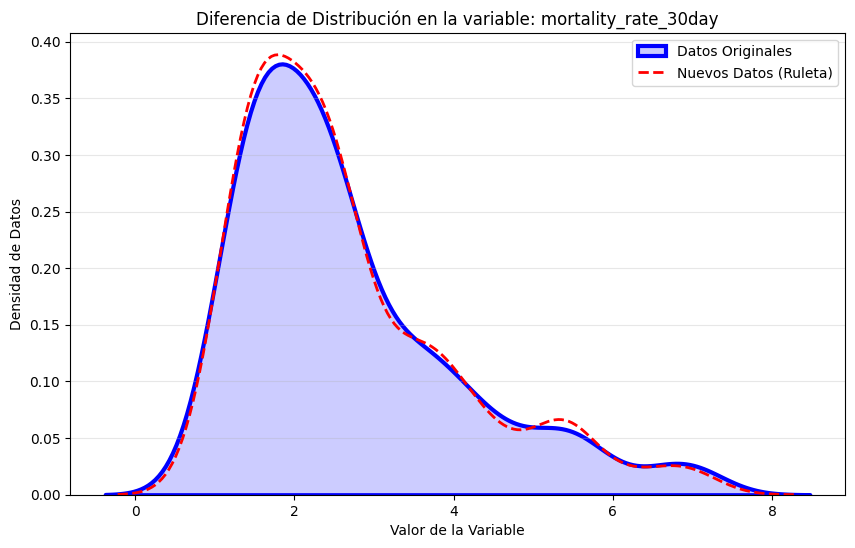
\includegraphics[width=\textwidth]{../Imagenes/Tarea3/Fase2_Mortalidad30dias.png}
         \caption{Mortalidad a 30 días}
     \end{subfigure}
     \hfill
     \begin{subfigure}[b]{0.32\textwidth}
         \centering
         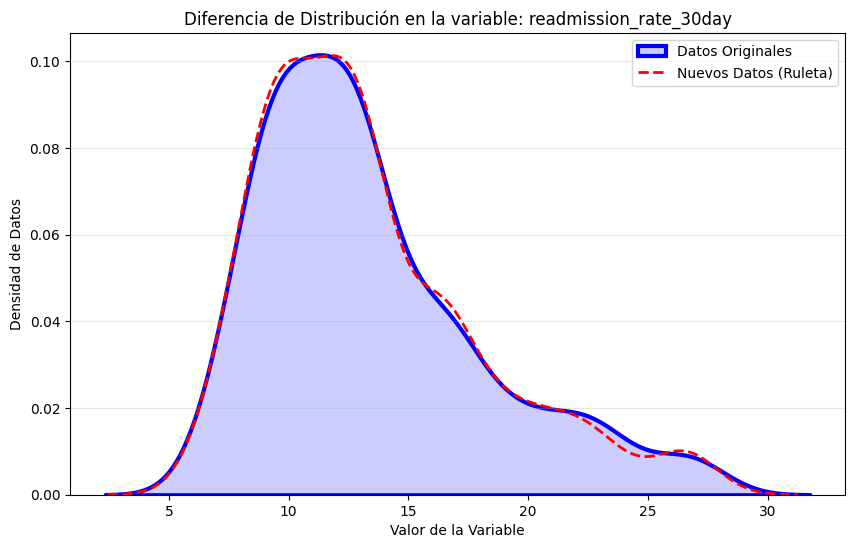
\includegraphics[width=\textwidth]{../Imagenes/Tarea3/Fase2_Readmision30dias.png}
         \caption{Tasa de Readmisión}
     \end{subfigure}
     \hfill
     \begin{subfigure}[b]{0.32\textwidth}
         \centering
         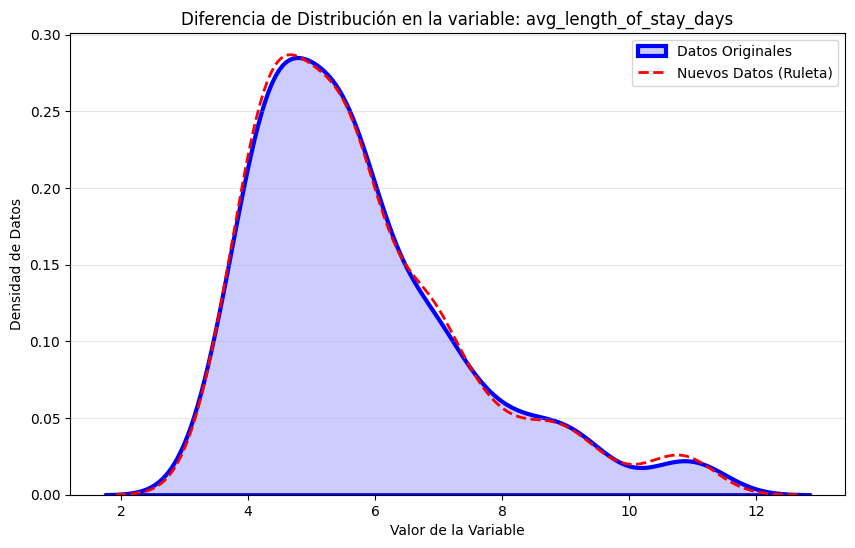
\includegraphics[width=\textwidth]{../Imagenes/Tarea3/Fase2_PromedioEstancia.png}
         \caption{Variable Adicional}
     \end{subfigure}
     \caption{Resultados consolidados de la Fase 2: Comparativa de densidades KDE con 300 registros sintéticos.}
     \label{fig:kde_fase2_completa}
\end{figure}

\subsection*{2. Conclusión de la Etapa de Equipo}
La Fase 2 confirma que el método propuesto es consistente. La desviación entre los datos originales y sintéticos es mínima, lo que garantiza que el aumento de datos no ha corrompido la realidad estadística del problema original, cumpliendo con los objetivos de representatividad institucional.

\section*{Fase 3: Integración Global y Validación Masiva (1200 registros)}

La etapa final del proyecto consistió en la consolidación de los datasets generados por todos los equipos del grupo, alcanzando un volumen total de \textbf{1200 registros sintéticos}. Esta fase permitió evaluar la robustez de la metodología de ruleta y sesgos hospitalarios a una escala masiva.

\subsection*{1. Análisis de Resultados: Convergencia Grupal}
Al contrastar el dataset integrado de 1200 registros contra el dataset original, se obtuvieron las siguientes conclusiones técnicas:

\begin{itemize}
    \item \textbf{Fidelidad Estadística Absoluta:} A diferencia de las fases anteriores, con 1200 registros las curvas de densidad (KDE) presentan una superposición casi total. La línea roja (sintética) sigue con precisión quirúrgica cada fluctuación de la línea azul (original), demostrando que el algoritmo es consistente a gran escala.
    \item \textbf{Estabilización de Variables Complejas:} Métricas como la tasa de complicaciones (\textit{complication\_rate}) y la estancia promedio (\textit{avg\_length\_of\_stay\_days}), que presentan distribuciones con sesgos específicos, fueron replicadas sin introducir anomalías o valores fuera de rango.
    \item \textbf{Reducción de la Varianza Inter-equipo:} La integración global permitió diluir pequeñas desviaciones individuales de las muestras de 150 y 300 datos, logrando un dataset sintético que funciona como un reflejo fiel de la población hospitalaria real.
\end{itemize}

\begin{figure}[H]
     \centering
     \begin{subfigure}[b]{0.31\textwidth}
         \centering
         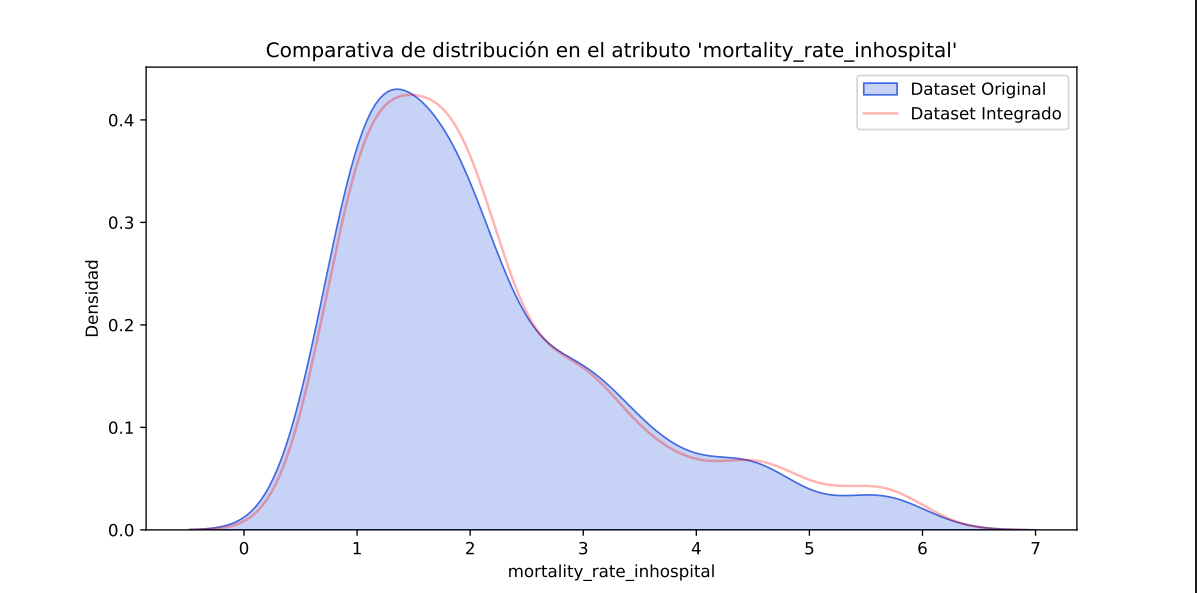
\includegraphics[width=\textwidth]{../Imagenes/Tarea3/Fase3_MortalityrateInHospital.png}
         \caption{Mortalidad Inhospitalaria}
     \end{subfigure}
     \hfill
     \begin{subfigure}[b]{0.31\textwidth}
         \centering
         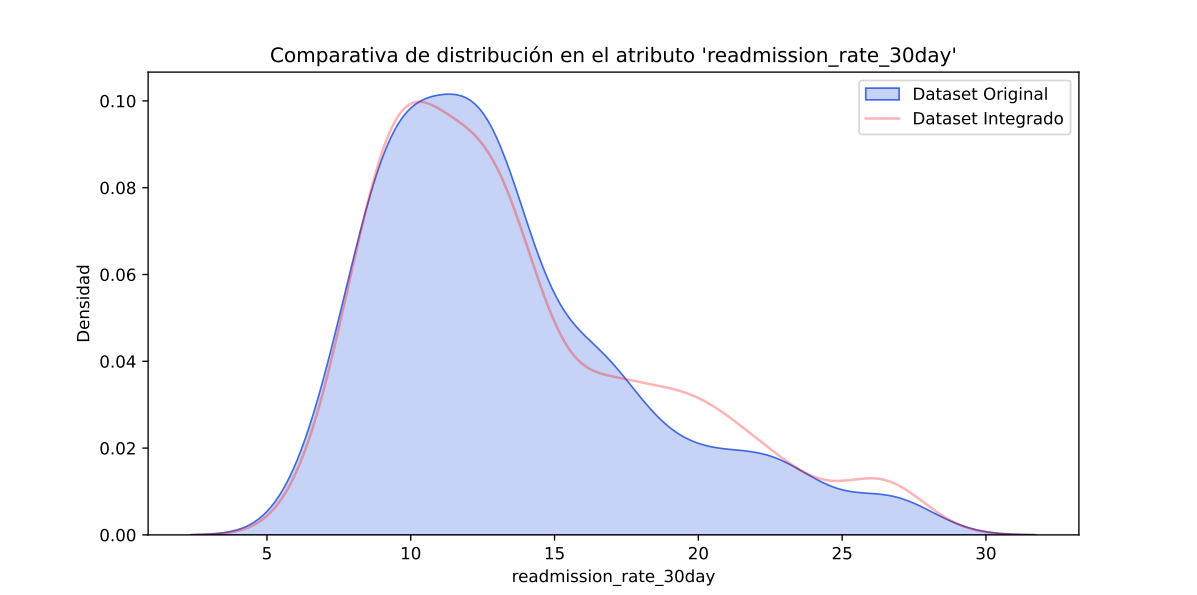
\includegraphics[width=\textwidth]{../Imagenes/Tarea3/Fase3_ReadmisionRate.png}
         \caption{Readmisión 30 días}
     \end{subfigure}
     \hfill
     \begin{subfigure}[b]{0.31\textwidth}
         \centering
         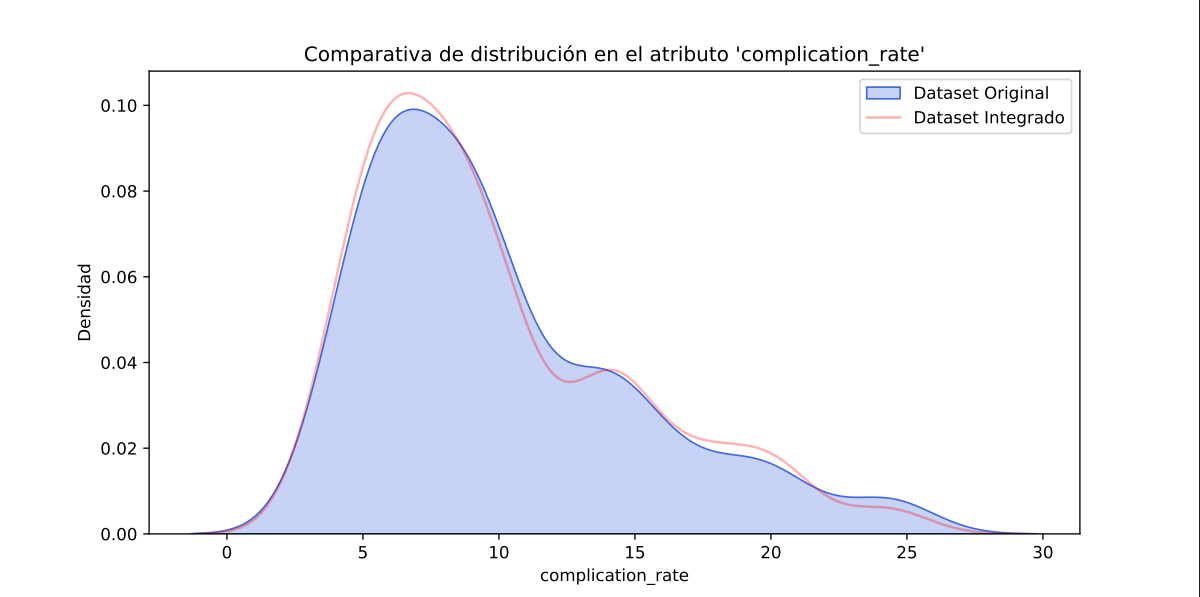
\includegraphics[width=\textwidth]{../Imagenes/Tarea3/Fase3_ComplicationRate.png}
         \caption{Tasa de Complicaciones}
     \end{subfigure}
     \caption{Resultados finales de la Fase 3: Comparativa global con 1200 registros. Se observa la máxima estabilidad en la distribución de las métricas clave.}
     \label{fig:fase3_global}
\end{figure}

\subsection*{2. Conclusión Final del Proceso de Síntesis}
El éxito de esta fase confirma que el uso de métodos probabilísticos controlados por diccionarios de sesgos institucionales permite generar datos sintéticos de alta calidad. El dataset final de 1200 registros es robusto, representativo y constituye una base sólida para el entrenamiento de modelos predictivos, garantizando la privacidad de los datos originales sin sacrificar la utilidad estadística.


\section{Conclusión}
El desarrollo de este proyecto confirma que el uso de métodos probabilísticos controlados por diccionarios de sesgos institucionales permite generar datos sintéticos de alta calidad. El proceso incremental de tres fases resultó fundamental para detectar y corregir desviaciones de manera temprana, logrando una transición fluida desde una muestra inicial de 150 registros hasta una base consolidada de 1200 datos con una convergencia estadística casi total.

Se concluye que el éxito del modelo radica en el equilibrio entre la aleatoriedad del algoritmo de ruleta y el cumplimiento estricto de los parámetros médicos predefinidos. El dataset final constituye una herramienta robusta, representativa y éticamente segura para el entrenamiento de futuros modelos de aprendizaje automático, garantizando la privacidad de los datos originales sin sacrificar la utilidad analítica necesaria para la toma de decisiones en el sector salud.


\printbibliography[title={Bibliográficas}]
\end{document}